% ============================================================================
%  4. PHƯƠNG PHÁP VÀ THỰC NGHIỆM
% ============================================================================
\section{Phương pháp và thực nghiệm}
\label{sec:phuong-phap}

\subsection{Kiến trúc tổng thể}

Hệ thống gồm ba tầng nối tiếp (Hình~\ref{fig:kien-truc}). \code{QueryAnalyzer} biến câu hỏi
tiếng Việt thành một biểu diễn hình thức $Q$; \code{InferenceEngine} dùng $Q$ để chọn bộ giải
và truy hồi tri thức từ \code{IndexedKnowledgeBase}; hàm sinh văn bản ghép câu trả lời kèm
căn cứ pháp lý. Tầng dense embedding là tuỳ chọn và mặc định không được gọi --- lý do trình
bày ở mục~\ref{sec:han-che}.

\begin{figure}[H]
\centering
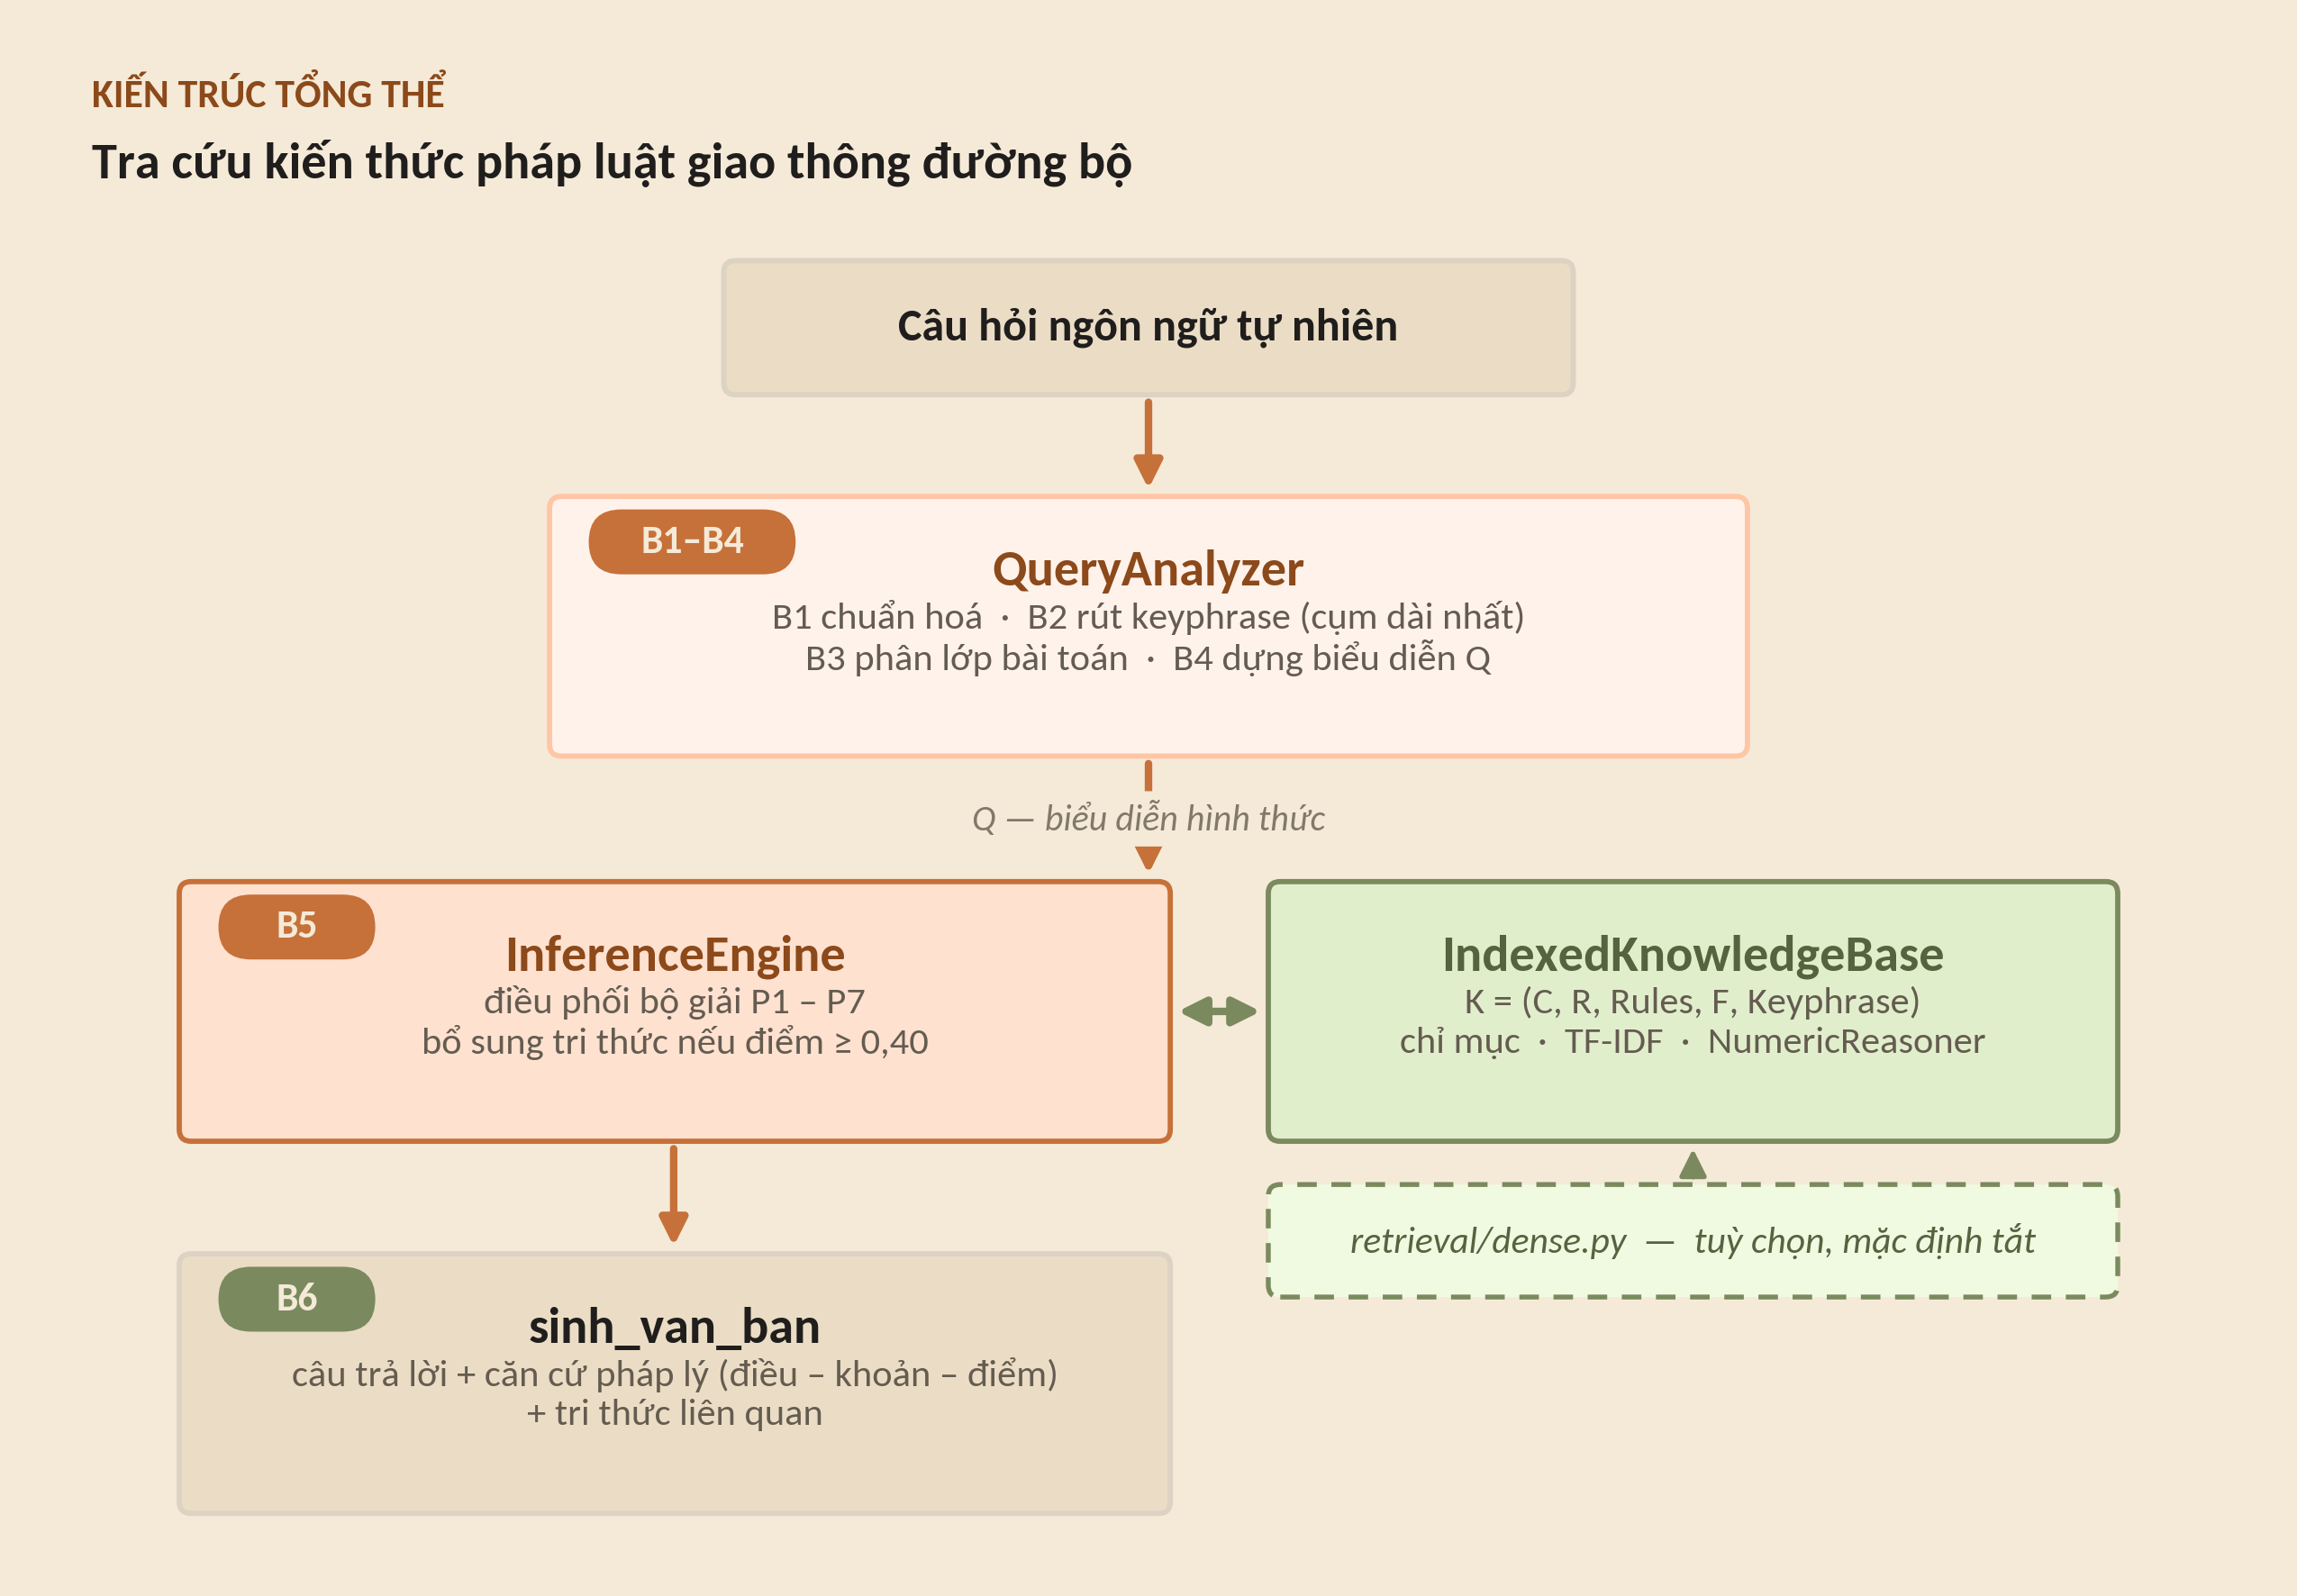
\includegraphics[width=0.96\textwidth]{figures/hinh1_kien_truc.png}
\caption{Kiến trúc hệ thống}
\label{fig:kien-truc}
\end{figure}

\subsection{Thuật giải xử lý truy vấn B1 -- B6}

\begin{table}[H]
\centering
\caption{Sáu bước xử lý một truy vấn}
\label{tab:b1-b6}
\renewcommand{\arraystretch}{1.2}
\begin{tabularx}{\textwidth}{@{}c >{\raggedright\arraybackslash}p{4.4cm} L@{}}
\toprule
\textbf{Bước} & \textbf{Việc} & \textbf{Hiện thực} \\
\midrule
B1 & Chuẩn hoá truy vấn         & Hạ chữ thường, chuẩn hoá Unicode, sinh bản không dấu \\
B2 & Rút trích keyphrase        & So khớp cụm dài nhất trên bản không dấu, không chồng lấn \\
B3 & Phân loại lớp bài toán     & Hàm điểm có trọng số trên sáu nhóm mẫu biểu thức chính quy \\
B4 & Dựng biểu diễn hình thức $Q$ & Keyphrase, nhóm, phương tiện, chủ thể, căn cứ, ràng buộc số \\
B5 & Suy diễn và truy hồi       & Bộ giải riêng cho từng lớp P1 -- P7 \\
B6 & Sinh câu trả lời           & Ghép nguyên văn điều khoản kèm căn cứ và tri thức liên quan \\
\bottomrule
\end{tabularx}
\end{table}

Thuật giải~\ref{alg:b1b6} mô tả toàn bộ quy trình ở mức giả mã.

\begin{algorithm}[H]
\small
\caption{Xử lý một truy vấn tra cứu pháp luật}
\label{alg:b1b6}
\KwIn{truy vấn $q$; mốc thời gian $t$; số kết quả $k$; cơ sở tri thức $K$}
\KwOut{$A(q,t) = (p, T, E)$}
$\hat q \leftarrow \mathrm{chuẩn\_hoá}(q)$;\quad $\bar q \leftarrow \mathrm{bỏ\_dấu}(\hat q)$ \tcp*{B1}
$KP \leftarrow \emptyset$;\quad $i \leftarrow 0$ \tcp*{B2: khớp cụm dài nhất}
\While{$i < |\bar q|$}{
  tìm $w \le 8$ lớn nhất sao cho cụm $\bar q[i..i{+}w)$ có trong từ điển $\mathit{Keyphrase}$\;
  \eIf{tìm thấy}{thêm cụm vào $KP$;\quad $i \leftarrow i + w$}{$i \leftarrow i + 1$}
}
$cc \leftarrow \mathrm{nhận\_dạng\_căn\_cứ}(\hat q)$;\quad $rb \leftarrow \mathrm{nhận\_dạng\_ràng\_buộc\_số}(\hat q)$\;
\eIf(\tcp*[f]{B3}){$cc \neq \emptyset$}{$p \leftarrow P6$}{$p \leftarrow \arg\max_{P}\ \mathrm{điểm\_lớp}(P \mid \bar q, KP, rb)$}
$Q \leftarrow (KP, \text{nhóm}, \text{phương tiện}, \text{chủ thể}, cc, rb)$ \tcp*{B4}
$T \leftarrow \mathrm{bộ\_giải}_p(Q, K)$, chỉ giữ $x$ có $t \in hl(x)$ \tcp*{B5}
\ForEach{loại tri thức còn thiếu trong $T$}{
  bổ sung các $x$ có $\mathrm{score}(x, q) \ge 0{,}40$\;
}
$E \leftarrow \{(\text{nguyên văn}(x), cc(x)) : x \in T\}$ \tcp*{B6}
\Return $(p,\ T[1..k],\ E)$\;
\end{algorithm}

Vì sao B2 phải khớp \emph{cụm dài nhất}: cụm ``nồng độ cồn'' phải thắng hai cụm rời ``nồng
độ'' và ``cồn''. Nếu khớp cụm ngắn trước, truy vấn sẽ trỏ sang mảng tri thức khác và mọi bước
sau đều sai theo.

\begin{figure}[H]
\centering
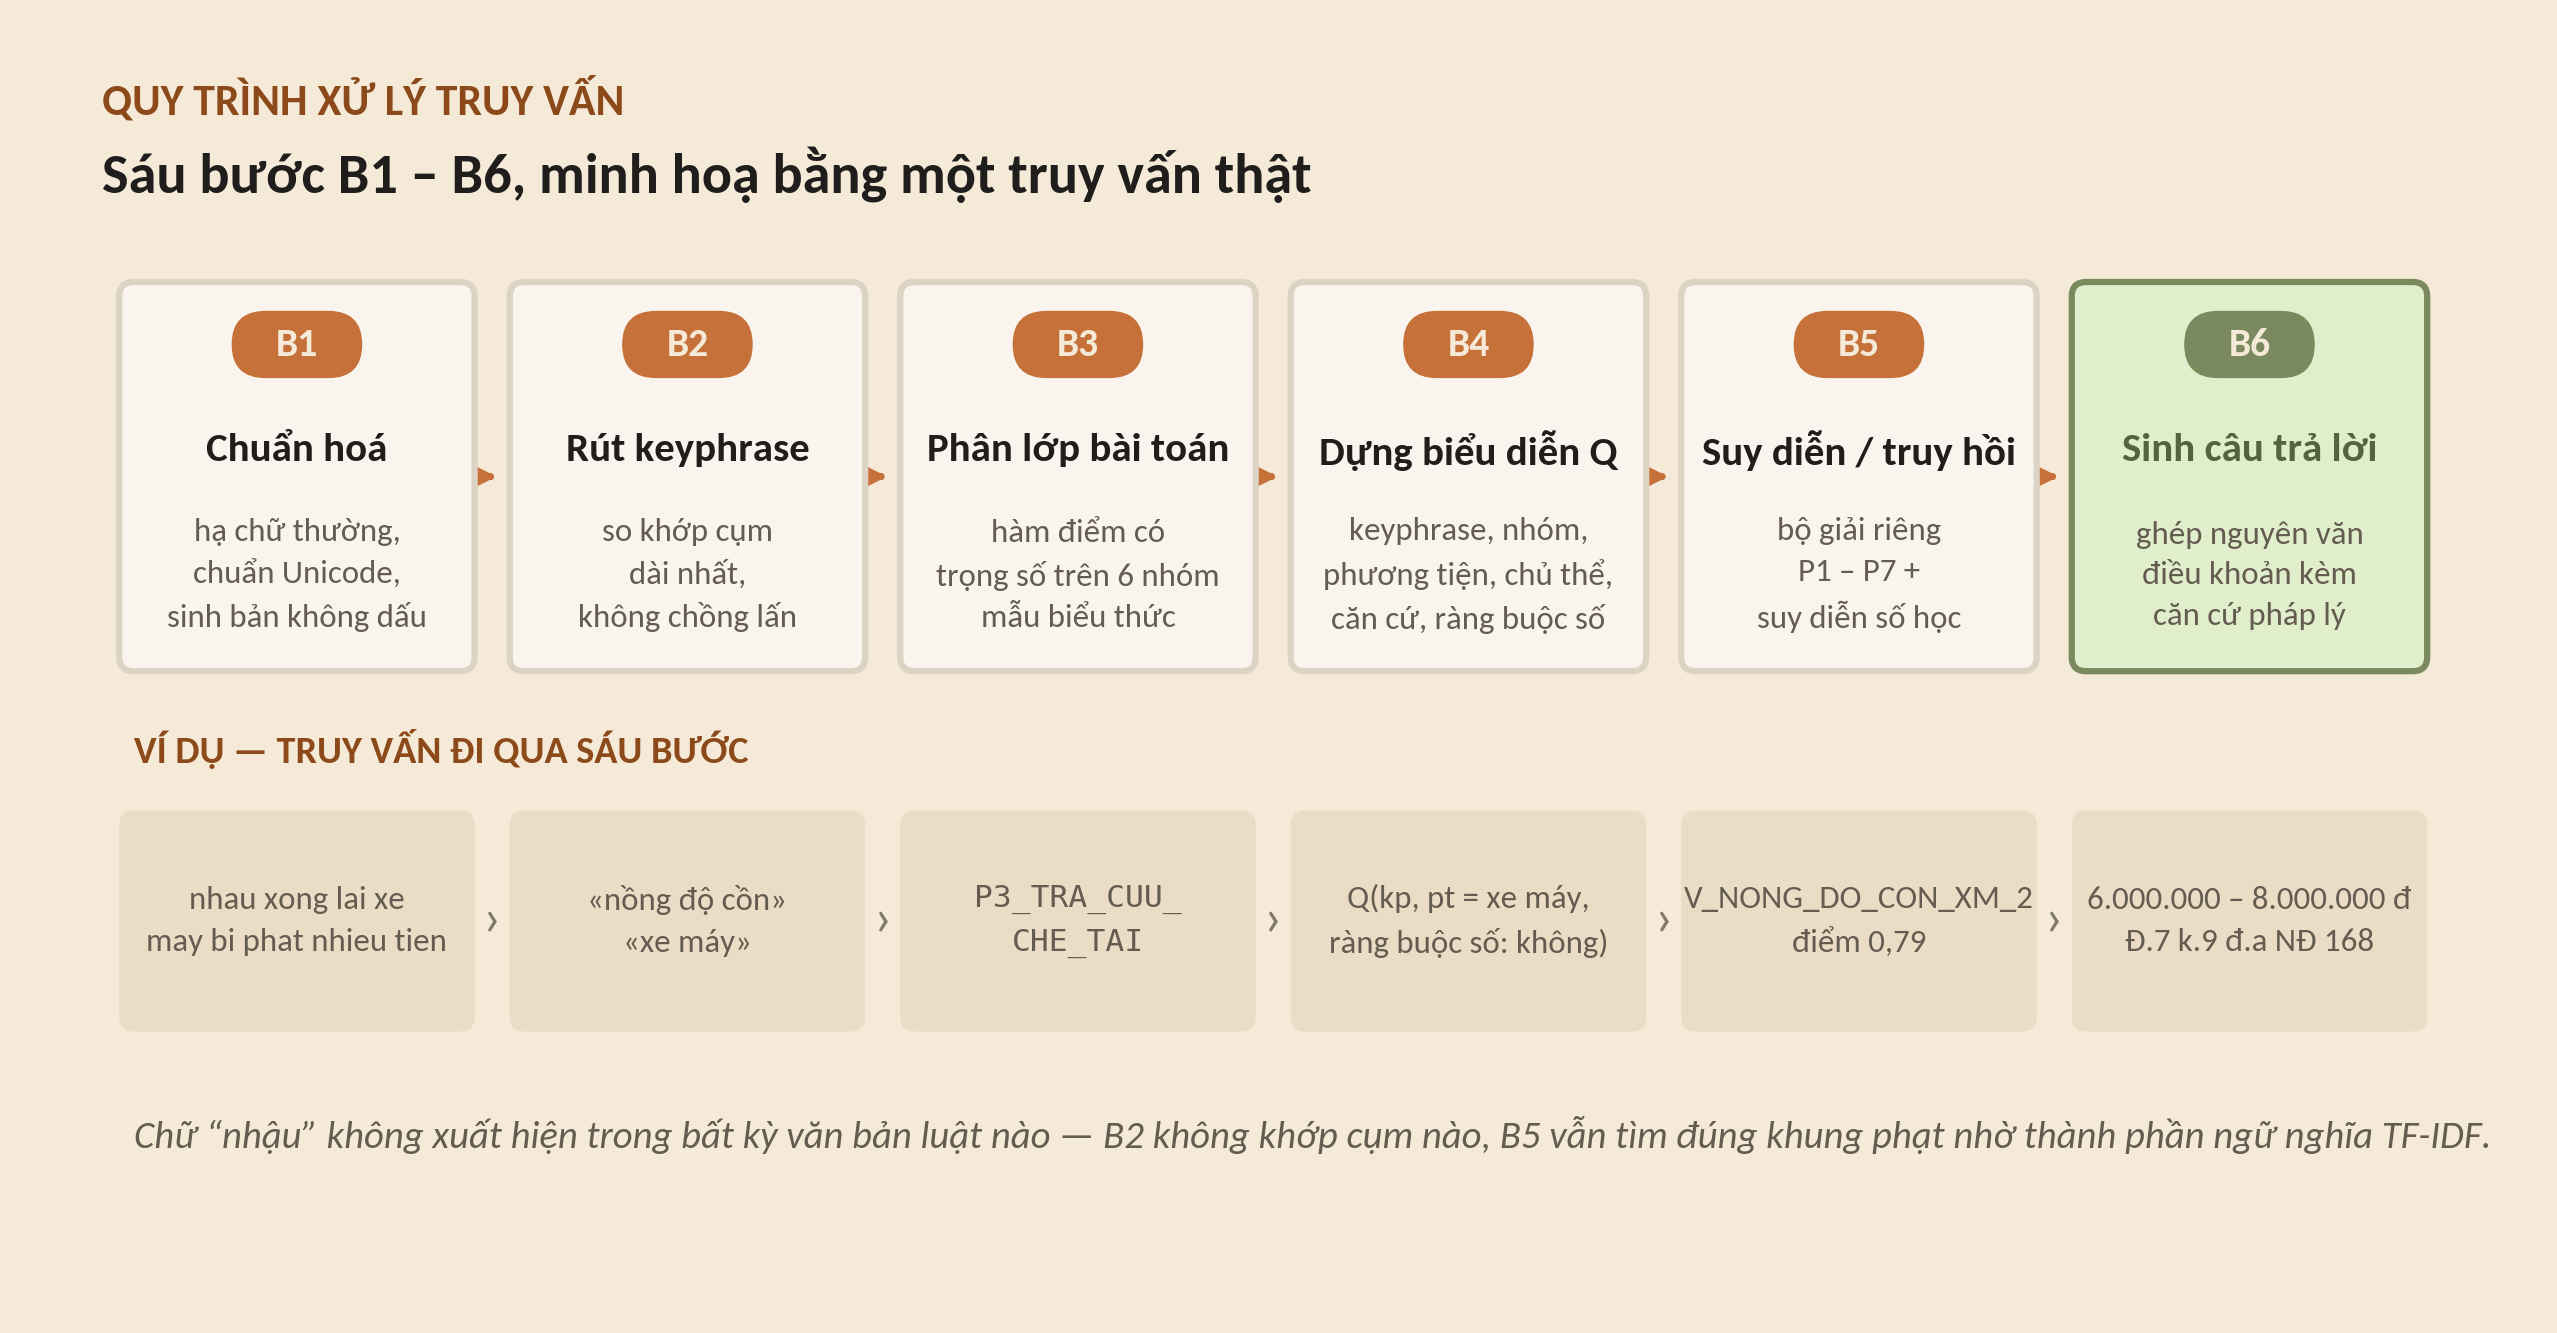
\includegraphics[width=0.9\textwidth]{figures/hinh2_luong_b1_b6.png}
\caption{Luồng xử lý truy vấn B1 -- B6 với một truy vấn thật}
\label{fig:luong}
\end{figure}

\subsection{Bảy lớp bài toán và bộ giải tương ứng}

\begin{table}[H]
\centering
\caption{Bảy lớp bài toán và câu hỏi tiêu biểu}
\label{tab:lop}
\renewcommand{\arraystretch}{1.2}
\begin{tabularx}{\textwidth}{@{}c >{\raggedright\arraybackslash}p{5.6cm} L@{}}
\toprule
\textbf{Lớp} & \textbf{Tên} & \textbf{Câu hỏi tiêu biểu} \\
\midrule
P1 & Tra cứu khái niệm, định nghĩa           & Xe cơ giới là gì? \\
P2 & Tra cứu quy định, quy tắc               & Quy tắc nhường đường tại nơi đường giao nhau? \\
P3 & Tra cứu chế tài                         & Vượt đèn đỏ xe máy phạt bao nhiêu? \\
P4 & Tra cứu ngược theo mức phạt / điểm trừ  & Lỗi nào bị trừ 10 điểm giấy phép lái xe? \\
P5 & Suy diễn tình huống nhiều hành vi       & Vừa vượt đèn đỏ vừa không có bằng thì tổng bao nhiêu? \\
P6 & Tra cứu theo căn cứ pháp lý             & Điều 6 khoản 9 điểm a NĐ 168/2024 nói về lỗi gì? \\
P7 & Tra cứu kiến thức liên quan             & Cho tôi thông tin về điểm giấy phép lái xe. \\
\bottomrule
\end{tabularx}
\end{table}

Điểm thiết kế đáng chú ý: \textbf{phân lớp không chặn kết quả}. Sau khi bộ giải của lớp được
chọn chạy xong, hệ thống vẫn bổ sung đủ ba loại tri thức (khái niệm, quy tắc, chế tài) nếu
còn thiếu và điểm vượt ngưỡng 0,40. Nhờ vậy một câu bị phân lớp sai vẫn có cơ hội trả đúng
--- đây chính là lý do Top-5 (95,00\%) cao hơn hẳn Top-1 (76,67\%).

\subsection{Hàm điểm lai}

Mỗi ứng viên tri thức $x$ được chấm theo
\begin{equation}
  \mathrm{score}(x, q) = \alpha \cdot s_{\text{keyphrase}}(x,q)
                       + \beta  \cdot s_{\text{ngữ nghĩa}}(x,q)
                       + \gamma \cdot s_{\text{ngữ cảnh}}(x,q)
  \label{eq:score}
\end{equation}
với $\alpha = 0{,}55$, $\beta = 0{,}30$, $\gamma = 0{,}15$.

\begin{table}[H]
\centering
\caption{Ba thành phần của hàm điểm và lý do chọn trọng số}
\label{tab:score}
\renewcommand{\arraystretch}{1.25}
\begin{tabularx}{\textwidth}{@{}>{\raggedright\arraybackslash}p{2.6cm} >{\raggedright\arraybackslash}p{5.0cm} L@{}}
\toprule
\textbf{Thành phần} & \textbf{Ý nghĩa} & \textbf{Vì sao trọng số đó} \\
\midrule
$s_{\text{keyphrase}}$ & Keyphrase trỏ thẳng tới định danh tri thức & Cao nhất (0,55) vì đây là tín hiệu chắc chắn: khớp đúng cụm từ pháp lý thì gần như không sai. \\
$s_{\text{ngữ nghĩa}}$ & Cosine TF-IDF char 3--5 gram kết hợp word 1--3 gram & 0,30 --- cứu các câu khẩu ngữ không có keyphrase, nhưng nhiễu hơn nên không được vượt keyphrase. \\
$s_{\text{ngữ cảnh}}$ & Khớp phương tiện, chủ thể, nhóm hành vi & 0,15 --- chỉ dùng để phân biệt các hành vi gần giống nhau, không đủ sức tự chọn kết quả. \\
\bottomrule
\end{tabularx}
\end{table}

Char $n$-gram chịu được lỗi chính tả và cách tách từ tiếng Việt; word $n$-gram giữ được cụm
nhiều từ. Với khái niệm và quy tắc, điểm ngữ nghĩa còn được trộn thêm 0,4 phần khớp riêng với
tên của mục tri thức: $s = 0{,}6\, s_{\text{nội dung}} + 0{,}4\, s_{\text{tên}}$.

\subsection{Suy diễn số học và hiệu lực theo thời gian}

Nhiều điều khoản phân khung theo ngưỡng số: nồng độ cồn chia ba mức, vượt tốc độ chia bốn
mức. So khớp từ khoá tìm ra đủ các khung nhưng không biết chọn khung nào.
\code{NumericReasoner} rút ngưỡng từ chính nguyên văn điều khoản thành một khoảng
$(a, b]$, so với giá trị $v$ trích từ câu hỏi và đẩy khung thoả $a < v \le b$ lên đầu.

\begin{keybox}
\textbf{Ví dụ.} \emph{``xe máy nồng độ cồn 0,3 mg/l phạt bao nhiêu''} $\Rightarrow$ $0{,}3$ thuộc
khung ``vượt quá 0,25 đến 0,4 miligam/1 lít khí thở'', không phải khung 0,25 hay khung trên
0,4. Hỏi liên tiếp 0,2 -- 0,3 -- 0,5 cho ba khung phạt khác nhau.
\end{keybox}

Về hiệu lực thời gian, mỗi mục tri thức mang khoảng $hl(x) = [\text{từ}, \text{đến})$ và mọi
truy vấn đều được lọc theo mốc $t$. Ví dụ quy tắc R15 về chở trẻ em dưới 10 tuổi mang nguyên
văn sau sửa đổi nên có hiệu lực từ 01/7/2026 theo Luật 118/2025, không phải 01/01/2025. Người
dùng đổi tham số \code{ngay=YYYY-MM-DD} là xem được cơ sở tri thức tại thời điểm đó.

\subsection{Cấu hình siêu tham số}

Toàn bộ siêu tham số được khai báo tường minh trong mã nguồn (hai tệp \code{engine.py} và \code{dense.py} nằm trong
thư mục \code{src/traffic\_law/}) và khoá lại bằng kiểm thử, không
có giá trị nào chỉnh ngầm lúc chạy.

\begin{table}[H]
\centering
\caption{Cấu hình siêu tham số của hệ thống}
\label{tab:sieu-tham-so}
\small
\renewcommand{\arraystretch}{1.2}
\begin{tabularx}{\textwidth}{@{}>{\raggedright\arraybackslash}p{3.5cm} >{\raggedright\arraybackslash}p{3.7cm} >{\raggedright\arraybackslash}p{2.1cm} L@{}}
\toprule
\textbf{Tham số} & \textbf{Giá trị} & \textbf{Vị trí} & \textbf{Ý nghĩa} \\
\midrule
ALPHA ($\alpha$) & 0,55 & \code{engine.py} & Trọng số làn keyphrase \\
BETA ($\beta$)   & 0,30 & \code{engine.py} & Trọng số làn ngữ nghĩa TF-IDF \\
GAMMA ($\gamma$) & 0,15 & \code{engine.py} & Trọng số làn ngữ cảnh \\
$k$ (top-$k$)    & 5    & tham số truy vấn           & Số kết quả trả về cho mỗi truy vấn \\
SUPPLEMENT\_\allowbreak THRESHOLD & 0,40 & \code{engine.py} & Ngưỡng bổ sung tri thức loại còn thiếu \\
Ngưỡng nhóm ngữ nghĩa & 0,24 · tối đa 2 nhóm & \code{engine.py} & Chặn suy đoán nhóm hành vi khi tín hiệu yếu \\
TF-IDF ký tự & \code{char\_wb}, $n$-gram 3--5, \code{sublinear\_tf} & \code{engine.py} & Chịu lỗi chính tả và cách tách từ \\
TF-IDF từ & \code{word}, $n$-gram 1--3, \code{sublinear\_tf} & \code{engine.py} & Giữ được cụm nhiều từ \\
Ngưỡng miền an toàn & 0,45 & \code{dense.py} & Giá trị lớn nhất còn giữ được cam kết không từ chối oan \\
Ngưỡng miền nghiêm ngặt & 0,52 & \code{dense.py} & Loại hết truy vấn rác nhưng từ chối oan --- không dùng mặc định \\
Mô hình dense (tuỳ chọn) & \code{paraphrase-}\newline\code{multilingual-}\newline\code{MiniLM-L12-v2} & \code{dense.py} & Chỉ bật khi cài gói tuỳ chọn, $\sim$470~MB \\
\bottomrule
\end{tabularx}
\end{table}

Hệ thống \textbf{không huấn luyện mô hình nào}: không có bước học tham số và không có tập huấn
luyện. Tuy vậy, cần nói rõ một điểm để không diễn giải quá số liệu: ba trọng số $\alpha, \beta,
\gamma$ được \emph{chọn và biện minh} bằng thí nghiệm loại bỏ thành phần
(mục~\ref{sec:ablation}) chạy trên \emph{chính} bộ 120 câu hỏi đánh giá. Bộ câu hỏi vì vậy vừa
là thước đo vừa là căn cứ để chọn cấu hình, và chưa có tập câu hỏi giữ lại (held-out) nào để
đo khả năng khái quát sang câu hỏi mới --- hạn chế này được ghi ở mục~\ref{sec:han-che}.

\subsection{Thiết lập thực nghiệm và chỉ số đo}
\label{sec:chi-so}

Bộ dữ liệu đánh giá gồm $N = 120$ câu hỏi; câu thứ $i$ có tập định danh đáp án chuẩn $G_i$,
lớp bài toán đúng và mức độ khó. Hệ thống trả về danh sách xếp hạng $T_i$ với $k = 5$ (riêng
lớp P4, P6 trả nguyên một tập thoả ràng buộc nên được chấm trên toàn tập). Ngoài ra có 40 truy
vấn ngoài lĩnh vực dùng để đo khả năng từ chối. Toàn bộ thực nghiệm chạy cục bộ, không gọi
dịch vụ ngoài.

Gọi $r_i$ là hạng của phần tử đúng đầu tiên trong $T_i$ ($r_i = \infty$ nếu không có). Các
chỉ số được tính như sau:
\begin{align}
  \text{Top-}n &= \frac{1}{N}\sum_{i=1}^{N} \mathbb{1}[\, r_i \le n \,],
  &
  \text{MRR} &= \frac{1}{N}\sum_{i=1}^{N} \frac{1}{r_i},
  \label{eq:topk-mrr}\\[2pt]
  P_i &= \frac{|G_i \cap T_i|}{|T_i|},\quad R_i = \frac{|G_i \cap T_i|}{|G_i|},
  &
  F1_i &= \frac{2 P_i R_i}{P_i + R_i},
  \label{eq:prf}
\end{align}
với precision, recall, F1 macro là trung bình của $P_i, R_i, F1_i$ trên $N$ câu. Khoảng tin cậy
95\% của một tỉ lệ $\hat p = x/n$ tính theo phương pháp Wilson:
\begin{equation}
  \frac{\hat p + \frac{z^2}{2n} \pm z\sqrt{\frac{\hat p(1-\hat p)}{n} + \frac{z^2}{4n^2}}}
       {1 + \frac{z^2}{n}}, \qquad z = 1{,}96.
  \label{eq:wilson}
\end{equation}
Để so hai cấu hình trên cùng bộ câu hỏi, dùng kiểm định McNemar chính xác: gọi $b$ là số câu
cấu hình mới đúng mà cấu hình cũ sai, $c$ là số câu ngược lại; khi đó
$p = \min\!\big(1,\ 2\sum_{j=0}^{\min(b,c)} \binom{b+c}{j} 2^{-(b+c)}\big)$.

\begin{table}[H]
\centering
\caption{Các chỉ số đo và ý nghĩa}
\label{tab:chi-so}
\renewcommand{\arraystretch}{1.2}
\begin{tabularx}{\textwidth}{@{}>{\raggedright\arraybackslash}p{4.3cm} L@{}}
\toprule
\textbf{Chỉ số} & \textbf{Đo điều gì} \\
\midrule
Độ chính xác phân lớp & Chất lượng bước B3 --- định tuyến tới đúng bộ giải \\
Top-1 / Top-3 / Top-5 & Chất lượng truy hồi ở các mức khoan dung khác nhau \\
MRR & Đáp án đúng thường nằm ở hạng nào \\
Precision / Recall / F1 (macro) & Độ sạch và độ phủ của tập trả về \\
Khoảng tin cậy 95\% (Wilson) & Độ bất định của mọi tỉ lệ do cỡ mẫu hữu hạn \\
Kiểm định McNemar & Chênh lệch giữa hai cấu hình có ý nghĩa thống kê hay không \\
AUC tách miền & Xác suất một câu hợp lệ được chấm cao hơn một truy vấn ngoài lĩnh vực \\
\bottomrule
\end{tabularx}
\end{table}
